%% ******************************************************
%% * This work may be distributed and/or modified under *
%% * the conditions of the LaTeX Project Public License *
%% *     http://www.latex-project.org/lppl.txt          *
%% * either version 1.3c of this license or any later   *
%% * version.                                           *
%% ******************************************************
\PassOptionsToPackage{quiet}{xeCJK}
\PassOptionsToPackage{quiet}{fontspec}
\PassOptionsToPackage{no-math}{fontspec}
\documentclass[11pt]{article}
\usepackage{geometry}
\usepackage{pdfpages}
\usepackage[level]{datetime}
\usepackage{unicode-math,xeCJK}
\usepackage{authblk}
\setmainfont{Libertinus Serif}
\setsansfont{Libertinus Sans}
\setmonofont{NotoSansMono}[
  Scale=MatchLowercase,
  Extension=.ttf,
  UprightFont=*-Light,
  BoldFont=*-Medium
]
\makeatletter
\usepackage{listings,dirtree}
\lstdefinestyle{TeX}{
    language      =  [LaTeX]TeX,
    texcsstyle    =  *\color{H7},
    numbers       =  none,
    basicstyle    =  {\small\color{H6}\tt},
    mathescape    =  false,
    breaklines    =  true,
    columns       =  fixed,
    keywordstyle  =  \color{H3},
    commentstyle  =  \color{darkgray},
    tabsize       =  2,
    keywords      =  {mail,flyleaf,sticker,logo,notebook,chapter,newnote,newnotesss,newnotessss,emptynote,newhdunote,
    makeframe,course,more}
}
\usepackage{hyperref,xcolor,verbatim}

\definecolor{pkgcolor}{Hsb}{103,.8,.5}
\definecolor{moducolor}{Hsb}{290,.8,.5}
\definecolor{cmdcolor}{Hsb}{188,.8,.5}
\definecolor{filecolor}{Hsb}{207,.6,.7}
\definecolor{H1}{Hsb}{349,.8,.8}% 海棠紅 (Hangzhou MTR L 1 )
\definecolor{H2}{Hsb}{23, .8,.8}% 丹桂橙 (Hangzhou Metro 2 )
\definecolor{H3}{Hsb}{48, .8,.8}% 柠檬黄 (Hangzhou Metro 3 )
\definecolor{H4}{Hsb}{103,.8,.8}% 香樟绿 (Hangzhou Metro 4 )
\definecolor{H5}{Hsb}{188,.8,.8}% 青藍色 (Hangzhou MTR L 5 )
\definecolor{H6}{Hsb}{207,.8,.8}% 海洋蓝 (Hangzhou Metro 6 )
\definecolor{H7}{Hsb}{290,.8,.8}% 浪漫紫 (Hangzhou Metro 7 )
\hypersetup{colorlinks,urlcolor=H1,linkcolor=H2,filecolor=filecolor,pdfstartview=FitH,pdfview=FitH,pdfcreator=XeTeX output}

\renewcommand*\l@subsection{\@dottedtocline{2}{1.5em}{2.1em}}
\def\pkg#1{\texorpdfstring{\textcolor{pkgcolor}{\textsf{#1}}}{“#1”}}
\def\mode#1{\texorpdfstring{\textcolor{moducolor}{\textsf{#1}}}{“#1”}}
\def\cmd#1{\texorpdfstring{\textcolor{cmdcolor}{\textsf{#1}}}{“#1”}}
\def\datechange#1#2{%
  \noindent{\makebox[\textwidth][r]{\color{H7}\rule{1.15\textwidth}{.4pt}}}
  \noindent\makebox[0pt][r]{\makebox[-3em][r]{\small\textbf{\textcolor{H7}{#1}}}\;\;}{\sffamily Update: \ignorespaces#2}}
\makeatother

\title{The \pkg{LiteTable} Template}
\author[1]{Xia Mingyu, \href{https://www.hdu.edu.cn}{Hangzhou Dianzi University}}
\yyyymmdddate
\date{\today}
\affil[1]{\href{mailto:xiamyphys@gmail.com}{\texttt{xiamyphys@gmail.com}}}
\date{\today\quad Version 2.2a\thanks{%
  \url{https://github.com/xiamyphys/litetable}}}
\begin{document}
\maketitle

\begin{abstract}
This is the document for \pkg{LiteTable} template, which provides a beautiful design of class schedule with colorful course blocks.

\end{abstract}

\tableofcontents

\section{Introduction}

\subsection{The purpose of this template}
This template provides a beautiful design of class schedule with colorful course blocks.

If you meet bugs when using this template, or you have better suggestions or ideas, or you want to participate in the development of the template or other templates by me, welcome to contact via email \href{mailto:xiamyphys@gmail.com}{xiamyphys@gmail.com}.

Also, you can join my \textsf\LaTeX{} Template Discussion \href{https://qm.qq.com/q/OnHzbNvVAG}{QQ Group: 760570712} to communicate with me and get the insider preview edition of the template.

\subsection{Packages required}
This template is based on the template \pkg{standalone}. And it requires \pkg{tikz} package to plot some graphics, \pkg{kvoptions} and \pkg{etoolbox} packages to provide global options, \pkg{expl3} package to support \cmd{timelist} array, \pkg{ctex} package to supports the \textbf{Chinese, Simplified} language and \pkg{fontawesome5} package to provides a set of beautiful icons.

I strongly suggest that you should use cmd to implement the commands to update all the packages to the latest version or switch to portable version instead.
\begin{verbatim}
    tlmgr update --self
    tlmgr update --all
\end{verbatim}

If you are in some areas with awful Internet environment, you can choose proper mirror source or use other means\footnote{Please comply with local network regulations.}. To learn more, please refer to \href{https://tex.stackexchange.com/questions/55437/how-do-i-update-my-tex-distribution}{How do I update my TEX distribution?}

\subsection{Loading \pkg{LiteTable} and its modes}
Save the file \verb|litetable.cls| to your project's root directory, and then create a \verb|.tex| file, just input the command \verb|\documentclass{litetable}| on the first line.

The template provides three modes, \mode{date}, \mode{style} and \mode{font}. Just add the options of the modes you want separately in the square bracket of the command \verb|\documentclass[options]{litetable}| in your \verb|.tex| file.

\newpage
\section{Modes of \pkg{LiteTable}}
\begin{verbatim}
  \documentclass[options]{litetable}
\end{verbatim}
\subsection{The \mode{date} mode}
This mode has two options, \mode{en} and \mode{cn}, which can make the weekdays display in English or 大陆简体, and the dafault option is English.

\subsection{The \mode{style} mode}
This mode has two options, \mode{round} and \mode{sharp}, which can make the course block's corners be round or sharp, and the default option is sharp.

\subsection{The \mode{font} mode}
This mode has two options, \mode{times} and \mode{libertinus}, which can make the font to be ``Times New Roman'' or ``Libertinus'', and the default option is ``Times New Roman''.\footnote{Please ensure that your computer has been already installed the font ``Libertinus'' when using this option.}

\section{Commands of \pkg{LiteTable}}

\subsection{The \cmd{makeframe} command}
\begin{verbatim}
    \makeframe{Timetable -- Semester 5}
\end{verbatim}

This command can create an empty class schedule with the title ``Timetable -- Semester 5''.

\subsection{The \cmd{timelist} command}
\begin{verbatim}
    \timelist{
      8:05,8:55,10:00,10:50,11:40,13:30,14:20,15:15,16:05,18:30,19:20,20:10;
      8:50,9:40,10:45,11:35,12:25,14:15,15:05,16:00,16:50,19:15,20:05,20:55
    }
\end{verbatim}

This command can add time to the left side of the timetable, and the first line of the content is the start time of the class while the second line of the content is the end time of the class, each time separates with comma (\verb|,|), the first line and the second line separates with semicolon (\verb|;|).

The timetable currently only supports 12 classes per day. In the future updates, customization of the number of courses per day will be supported.

\subsection{The \cmd{course} command}
\begin{verbatim}
    \course{H5}{3}{5}{AQM}{Building 6·225}{Yuan Li \& Mengnan Chen}{Week 1 -- 18}
\end{verbatim}

There are 7 variables in this command.
\begin{itemize}
  \item The 1st one is the color of the class that you want, from ``H1'' to ``H5''.
  \item The 2nd and 3rd ones is the starting number and ending number of the class.
  \item The 4th one is the name of the class.
  \item The 5th one is the address of the class.
  \item The 6th one is the name of the teacher(s).
  \item The last one is the start week and end week of the class.
\end{itemize}

\subsection{The \cmd{newday} command}
This command can switch the current weekday to the next day, then the course will move right one grid.

\subsection{The \cmd{more} command}
\begin{verbatim}
  \more{·School Start: 04 / 03 / 2024 ·Summer Vacation: 05 / 07 / 2024}
\end{verbatim}
This command can add remark at the end of the class schedule.

\subsection{The \cmd{sticker} command}
\begin{verbatim}
  \sticker{favicon}
\end{verbatim}
There will be a sticker on the southeast of the page after you add,otherwise it won't.

\newpage
\section{Version History}

The design of this course schedule originated from the student course schedule web page\footnote{Only those studying at or graduated from Hangzhou Dianzi University can have the permission of access.} of the \href{https://www.hduhelp.cn/}{HDUHelp} in \href{https://www.hdu.edu.cn}{Hangzhou Dianzi University}\footnote{https://en.wikipedia.org/wiki/Hangzhou\_Dianzi\_University}. The layout is very beautiful and then I used \LaTeX{} to imitate that style and made a class schedule template to share with everyone.

\textsf{\bfseries Version 1.0} was finished on 1 September, 2023 and released on \href{https://www.latexstudio.net/index/details/index/mid/3625.html}{LaTeX Studio} (Xiaoshan, Hangzhou) and \href{http://xhslink.com/od7Ycw}{Xiaohongshu}, where won the favor of many people.

\textsf{\bfseries Version 2.0a} was finished developing on 1 November, 2023 and released on \href{https://www.latexstudio.net/index/details/index/mid/3636.html}{LaTeX Studio} (Xiaoshan, Hangzhou) and \href{http://xhslink.com/od7Ycw}{Xiaohongshu}. This version used \verb|.cls| files to make the \verb|main.tex| file more concise. Also, this version have added a global option to choose whether the corners of the ``course Block" to be round or sharp. And this version support adds multiply class schedules in one \verb|.tex| file.

\textsf{\bfseries Version 2.1a} was finished developing on 5 November, 2023. Supports the libertinus font.

\textsf{\bfseries Version 2.2a} was finished developing on 31 January, 2024. This Version fixed the bug of resolution exceeded, changed paper type to US letter and support custom course start time and end time.

\datechange{01/09/2023}{Version 2.0a}
\begin{itemize}
    \item Supports the course block's corners be round or sharp.
    \item Supports multiply class schedules in one \verb|.tex| file.
\end{itemize}

\datechange{05/11/2023}{Version 2.1a}
\begin{itemize}
    \item Supports the libertinus font.
\end{itemize}

\datechange{31/01/2024}{Version 2.2a}
\begin{itemize}
    \item Fixed the bug of resolution exceeded.
    \item Changed paper type to US letter.
    \item Support custom course start time and end time.
    \item Support add sticker as you like at the southeast of the page.
\end{itemize}

\newpage
\appendix
\section{Document Example}
\lstinputlisting[style=TeX]{litetable-demo.tex}

\includepdf[pages=last-1,nup=1x2,angle=90]{litetable-demo.pdf}
\end{document}